\documentclass[12pt, twoside]{article}
\usepackage[letterpaper, margin=1in, headsep=0.5in]{geometry}
\usepackage[english]{babel}
\usepackage[utf8]{inputenc}
\usepackage{amsmath}
\usepackage{amsfonts}
\usepackage{amssymb}
\usepackage{tikz}
\usetikzlibrary{quotes, angles}
\usepackage{graphicx}
\usepackage{enumitem}
\usepackage{multicol}

\newif\ifmeta
\metatrue %print standards and topics tags

\title{Regents Geometry}
\author{Chris Huson}
\date{September 2020}

\usepackage{fancyhdr}
\pagestyle{fancy}
\fancyhf{}
\renewcommand{\headrulewidth}{0pt} % disable the underline of the header
\raggedbottom


\fancyhead[LE]{\thepage}
\fancyhead[RO]{\thepage \\ Name: \hspace{4cm} \,\\}
\fancyhead[LO]{BECA / Dr. Huson / Geometry 09-Congruence-transformations\\* pset ID: 150}

\begin{document}

\subsubsection*{9-3CW-SSA}
\begin{enumerate}
\item 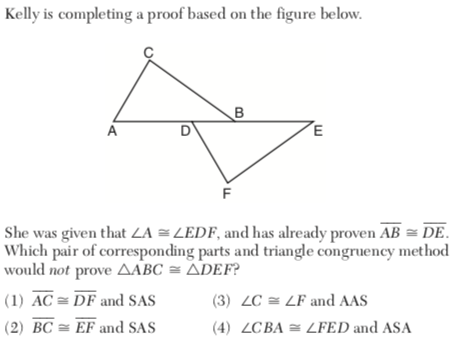
\includegraphics[scale=0.8]{geom-62017-9.png}
\item Sketch the triangles first. \\
    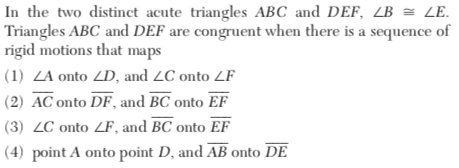
\includegraphics[scale=0.8]{geom-62017-22.png}
\item Sketch the triangles first. \\
      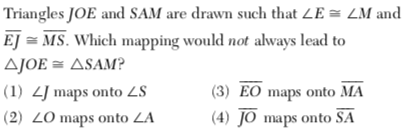
\includegraphics[scale=0.8]{geom-62019-14.png}
\item 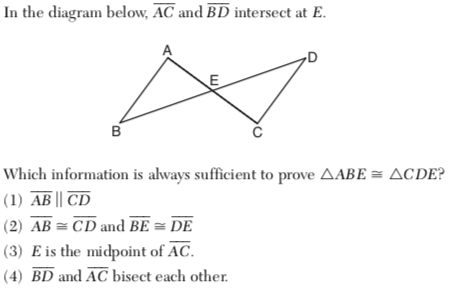
\includegraphics[scale=0.8]{geom-62019-8.png}
\item Sketch the triangles first. \\
      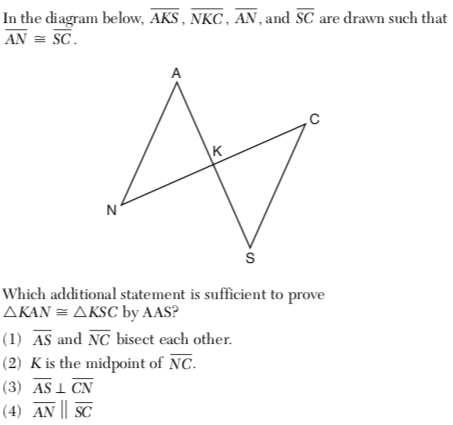
\includegraphics[scale=0.8]{geom-82019-10.png}

\end{enumerate}
\end{document}